\documentclass[12pt,a4paper]{report}

% --- Paquets bàsics ---
\usepackage[catalan]{babel}
\usepackage[utf8]{inputenc}
\usepackage[T1]{fontenc}
\usepackage{lmodern}
\usepackage{geometry}
\usepackage{setspace}
\usepackage{graphicx}
\usepackage[hidelinks]{hyperref}
\usepackage{amsmath}
\usepackage{amsfonts}
\usepackage{amssymb}
\usepackage{float}
\usepackage{listings}
\usepackage{xcolor}
\usepackage{caption}

\lstdefinelanguage{CSharp}{
  language=[Sharp]C
}

\lstset{
  basicstyle=\ttfamily\footnotesize,
  breaklines=true,
  breakatwhitespace=false,
  postbreak=\mbox{\textcolor{red}{$\hookrightarrow$}\space},
  captionpos=b,
  frame=single,
  framerule=0.5pt,
  rulecolor=\color{gray!60},
  aboveskip=6pt,
  belowskip=6pt,
  keywordstyle=\color{blue},
  commentstyle=\color{gray},
  stringstyle=\color{teal},
  showstringspaces=false,
  tabsize=2
}
\begin{document}


\chapter{Pantalles HMI amb Rapid SCADA}

Continuant amb els conceptes de comunicació mitjançant MQTT i la integració amb Rapid SCADA descrits en l'apartat anterior, en aquesta secció es detalla com es dissenyen les pantalles HMI que permeten visualitzar i interactuar amb les variables del sistema.

L'objectiu principal d'aquestes pantalles és oferir una interfície clara i intuïtiva que permeti:
\begin{itemize}
    \item Visualitzar l'estat del sistema en temps real
    \item Interpretar el comportament dels sensors i actuadors
    \item Interactuar amb el procés industrial simulat
\end{itemize}

\textit{Aclaració: tots els elements visuals referents a imatges que s'observen en les diferents pantalles s'han generat amb Intel·ligència Artificial}
\section{Estructura de les vistes en Rapid SCADA}

Per a la creació de pantalles, Rapid SCADA utilitza el mòdul \textit{Views} \cite{rapidscada_views}, des del qual es poden generar diferents tipus d'arxius visuals accessibles per l'usuari.

Inicialment, es va crear una vista de tipus \texttt{.tbl} anomenada \textit{VistaPlanta}, amb l'objectiu de visualitzar totes les variables del sistema a través dels canals configurats. Aquesta vista permetia observar en temps real els valors dels tòpics MQTT, però presentava una limitació important: la manca d'una representació visual intuïtiva.

Per aquest motiu, es van desenvolupar tres pantalles HMI específiques orientades a millorar la visualització i el control del sistema.

Pel que fa a la navegació entre pantalles, aquesta es realitza exclusivament mitjançant el menú predefinit de Rapid SCADA. L'eina no permet implementar una estructura de navegació interna personalitzada dins de les pròpies vistes, fet que limita la flexibilitat en el disseny de la interfície d'usuari.

\section{Pantalla de visualització de sensors}

Aquesta pantalla (figura \ref{fig:pantalla_sensors}) està orientada exclusivament a la monitorització del sistema, sense capacitat d'interacció directa.

Per al seu desenvolupament s'ha utilitzat el format \texttt{.sch} (\textit{ScadaSchemeEditor}), que permet incloure elements gràfics com textos, imatges i indicadors dinàmics.

\subsection{Funcionament general}

Les dades generades a Unity (com sensors de presència, posició o comptadors) són publicades mitjançant MQTT i rebudes a Rapid SCADA a través dels canals d'entrada. Aquesta pantalla permet visualitzar en temps real l'estat d'aquestes variables, facilitant la comprensió del comportament del sistema.

\subsection{Elements utilitzats}

\begin{itemize}
    \item \textbf{Static Text}: utilitzat per títols i etiquetes fixes.
    \item \textbf{Dynamic Text}: mostra valors en temps real associats a canals.
    \item \textbf{Dynamic Image}: element clau per representar visualment l'estat de sensors i actuadors.
\end{itemize}

Els \textit{Dynamic Text} s'associen a un canal d'entrada (\textit{input channel}), mostrant en tot moment el valor actual publicat al tòpic MQTT corresponent. Aquest element és útil per representar els comptadors dintre de les nostres pantalles, sabent el seu valor en temps real \cite{RapidScadaVideos} . 


El component més rellevant és el \textit{Dynamic Image} , que permet canviar la imatge en funció del valor rebut:

\begin{itemize}
    \item Sensors binaris: dues imatges (0 = apagat, 1 = activat) (figura \ref{fig:sensor_estat})
    \item Motors: estat actiu/inactiu (figura \ref{fig:motor_estat1})
    \item Rodets: tres estats (stop, forward, reverse) (figura \ref{fig:motor_estat2})
    \item Sensor òptic: imatge segons el tipus de peça detectada, treta de la simulació realitzada en Unity. 
\end{itemize}

\subsection{Representació gràfica dels elements}

A continuació es mostren exemples representatius dels diferents tipus d'elements visuals utilitzats i una imatge de la vista general de la pantalla:

\begin{figure}[H]
    \centering
    
\includegraphics[width=0.1\linewidth]{images/sensor_off.png}
    
\includegraphics[width=0.1\linewidth]{images/sensor_on.png}
    \caption{Representació d'un sensor en estat apagat i activat}
    \label{fig:sensor_estat}
\end{figure}

\begin{figure}[H]
    \centering
    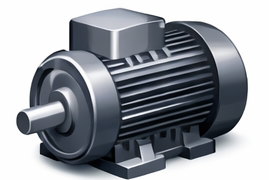
\includegraphics[width=0.1\linewidth]{images/motor_off.png}
    
\includegraphics[width=0.1\linewidth]{images/motor_on.png}
    \caption{Representació d'un motor en estat inactiu i actiu}
    \label{fig:motor_estat1}
    \centering
    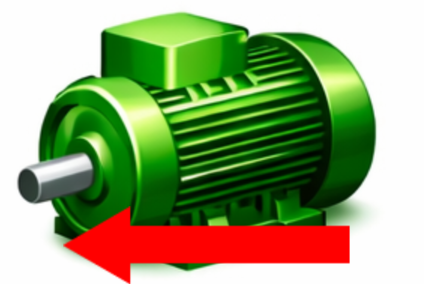
\includegraphics[width=0.1\linewidth]{images/motor_forward.png}
    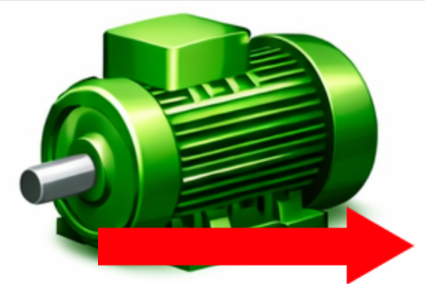
\includegraphics[width=0.1\linewidth]{images/motor_reverse.png}
    \caption{Estats dels rodets: parat, endavant i enrere}
    \label{fig:motor_estat2}
\end{figure}

\subsection{Vista general de la pantalla}


\begin{figure}[H]
    \centering
    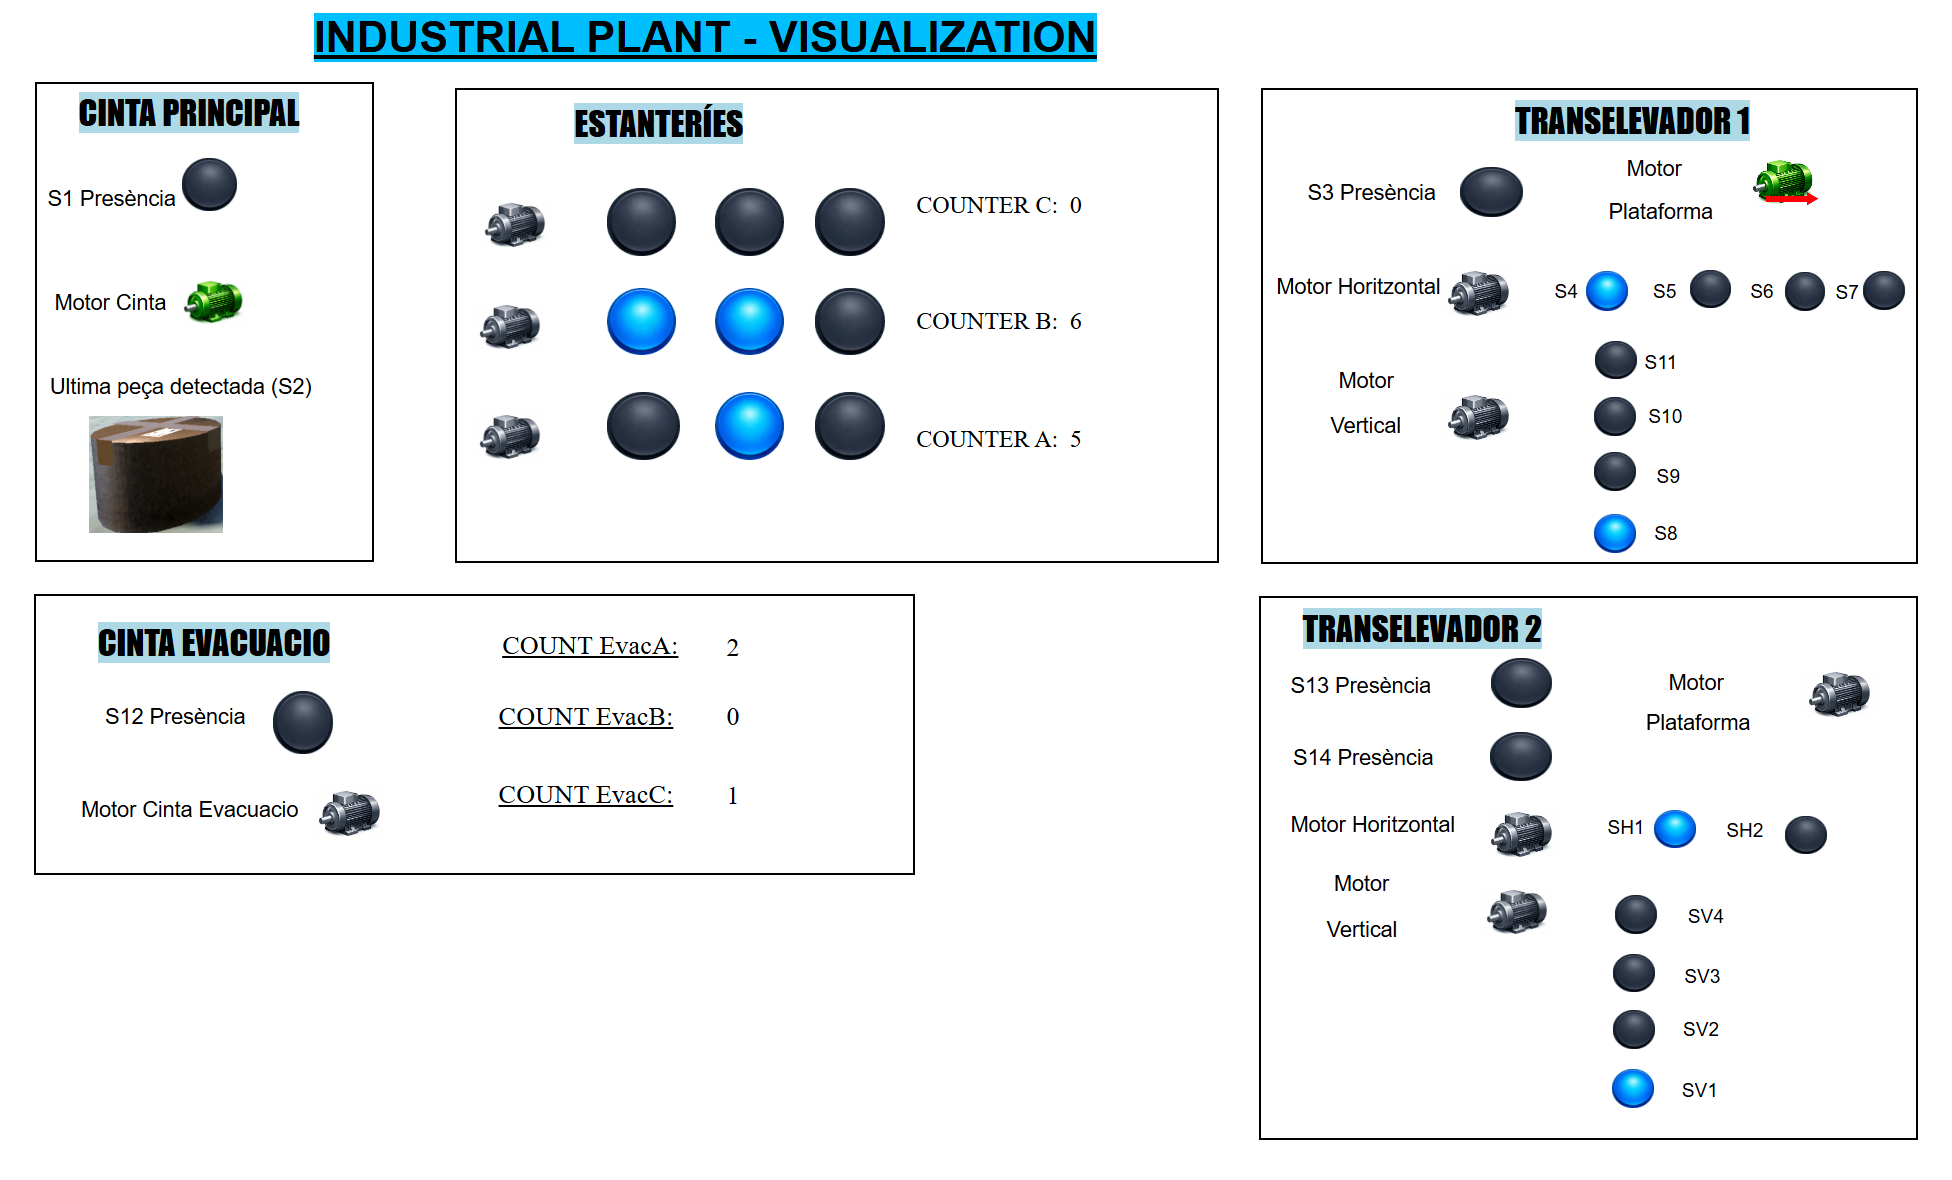
\includegraphics[width=0.9\linewidth]{images/pantalla_sensors.png}
    \caption{Pantalla de visualització de sensors}
    \label{fig:pantalla_sensors}
\end{figure}


\section{Pantalla de control del procés}

La segona pantalla està orientada al control del sistema i permet enviar comandes als actuadors (figura \ref{fig:main_screen}).

Per a la seva implementació s'ha utilitzat el tipus \textit{Mimic Diagram}, que requereix la instal·lació d'un plugin específic de Rapid SCADA.

\subsection{Tecnolgía utilitzada: Mimic Diagram}

A diferència del format \texttt{.sch}, el Mimic Diagram \cite{RapidScadaMimicVideo} permet enviar comandes directament als canals mitjançant la funcionalitat \textit{Send Command}, facilitant la interacció amb el sistema.

\subsection{Elements de control}

Aquesta pantalla inclou:

\begin{itemize}
    \item Botons de \textbf{Start} i \textbf{Stop}
    \item Selector de mode (Manual / Automàtic / Neutre)
    \item Botó d'\textbf{Emergència}
    \item Botó de \textbf{Reset}
    \item Botó de \textbf{Pause} 
\end{itemize}

\subsection{Implementació dels elements interactius}
\subsubsection{Selector de mode}

El selector de mode s'ha implementat mitjançant:
\begin{itemize}
    \item Un element visual amb \textit{input channel} (estat actual)
    \item Tres zones invisibles superposades que envien comandes segons la posició seleccionada
\end{itemize}

Aquest mètode permet simular un selector físic dins de l'entorn HMI (figura \ref{fig:selector_mode}). La imatge del selector està vinculada a un \textit{input channel}, de manera que mostra en tot moment l'últim valor assignat a aquest element.

\begin{figure}[H]
\centering
\begin{minipage}{0.32\textwidth}
    \centering
    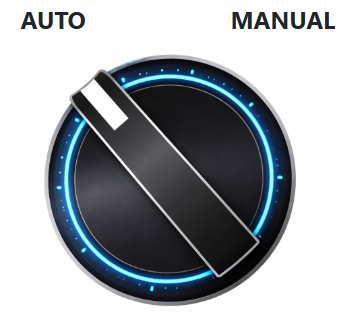
\includegraphics[width=\linewidth]{images/selector_0.png}
    \caption*{Mode automàtic}
\end{minipage}
\begin{minipage}{0.32\textwidth}
    \centering
    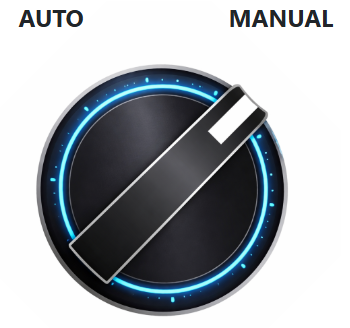
\includegraphics[width=\linewidth]{images/selector_1.png}
    \caption*{Mode manual}
\end{minipage}
\begin{minipage}{0.32\textwidth}
    \centering
    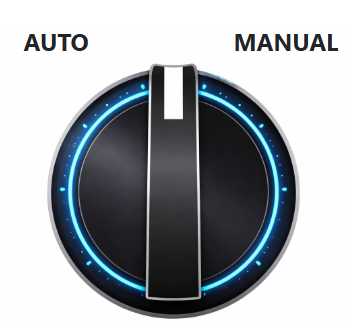
\includegraphics[width=\linewidth]{images/selector_-1.png}
    \caption*{Mode emergència}
\end{minipage}
\caption{Posicions del selector de mode}
\label{fig:selector_mode}
\end{figure}

\subsubsection{Botons de control}

Durant la implementació de la pantalla de control, es va observar que alguns botons (com Start, Stop o Emergència) presentaven un comportament unidireccional, és a dir, permetien enviar un valor però no gestionar correctament el canvi d'estat.

Per solucionar aquesta limitació \cite{RapidScadaVideos}, es va implementar una tècnica basada en l'ús de \textbf{toggles invisibles} superposats als elements de control. Cada botó es va associar a un canal configurat com a \textit{input} i \textit{output}, permetent conèixer en tot moment el seu estat.

El funcionament consisteix en un botó visual amb una imatge dinàmica vinculada al canal, sobre el qual es col·loca un toggle invisible que, en ser activat, envia el valor contrari a l'estat actual. D'aquesta manera, s'aconsegueix un comportament bidireccional coherent amb la representació gràfica del botó.

Tot i això, aquesta solució presenta una limitació respecte als sistemes industrials reals. Habitualment, botons com \textbf{Start} i \textbf{Stop} són de tipus momentani,és a dir, només estan actius mentre es mantenen premuts, retornant automàticament al seu estat inicial, mentre que altres com el d'\textbf{Emergència} són biestables. En el Mimic Diagram no s'ha pogut reproduir aquest comportament de forma directa, de manera que tots els botons s'han implementat com a biestables.

Aquesta simplificació pot generar situacions no desitjades, com l'activació simultània de \textbf{Start} i \textbf{Stop}, fet que s'ha resolt a nivell de control mitjançant la lògica definida en el GRAFCET (Figura \ref{fig:botons_control}).


\begin{figure}[H]
\centering
\begin{minipage}{0.42\textwidth}
    \centering
    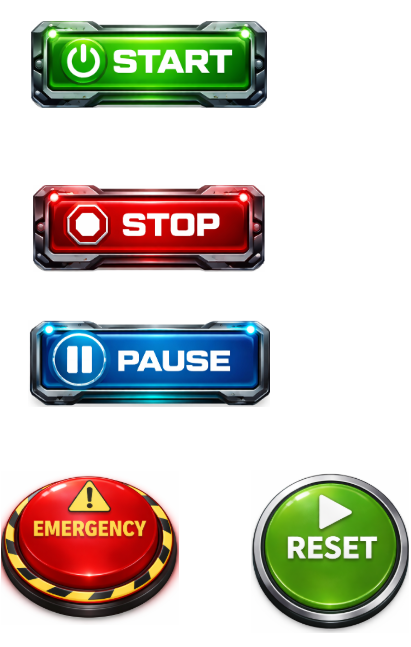
\includegraphics[width=\linewidth]{images/botons_no.png}
    \caption*{Botons en estat inactiu}
\end{minipage}
\hfill
\begin{minipage}{0.44\textwidth}
    \centering
    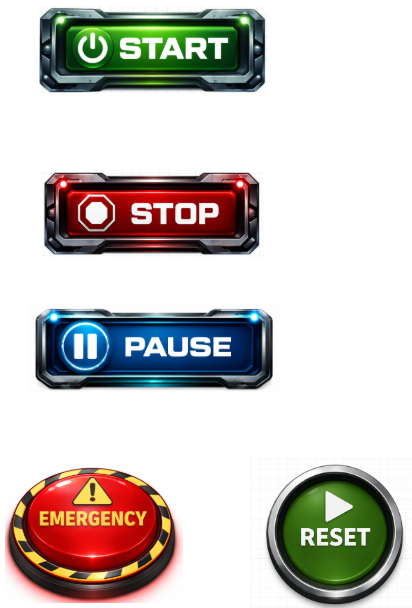
\includegraphics[width=\linewidth]{images/botons_si.png}
    \caption*{Botons en estat actiu}
\end{minipage}
\caption{Comparativa dels estats dels botons de control}
\label{fig:botons_control}
\end{figure}


\subsection{Indicadors visuals}

La pantalla també incorpora indicadors lluminosos que mostren el mode específic en el que es troba el sistema de la planta industrial (emergència, manual o automàtic, figura \ref{fig:indicadors_mode}), acompanyat de 3 textos que apareixen o desapareixen en concordancia amb el mode actiu. 

\begin{figure}[H]
\centering
\begin{minipage}{0.32\textwidth}
    \centering
    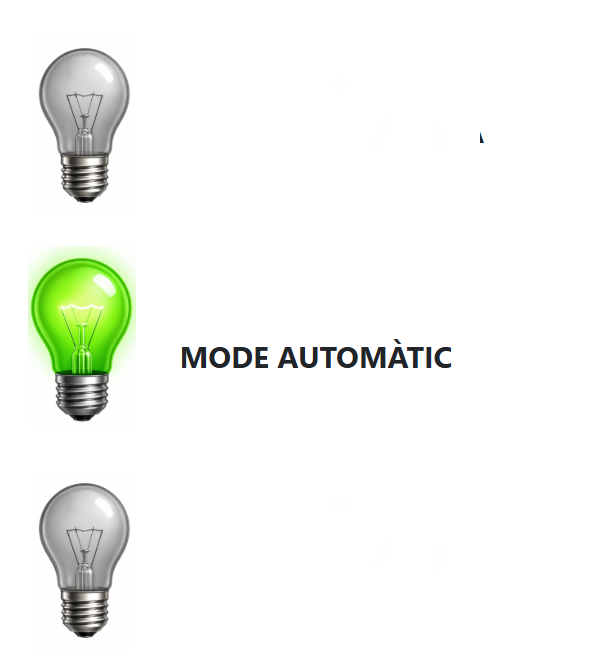
\includegraphics[width=\linewidth]{images/light_auto.png}
    \caption*{Mode automàtic}
\end{minipage}
\begin{minipage}{0.32\textwidth}
    \centering
    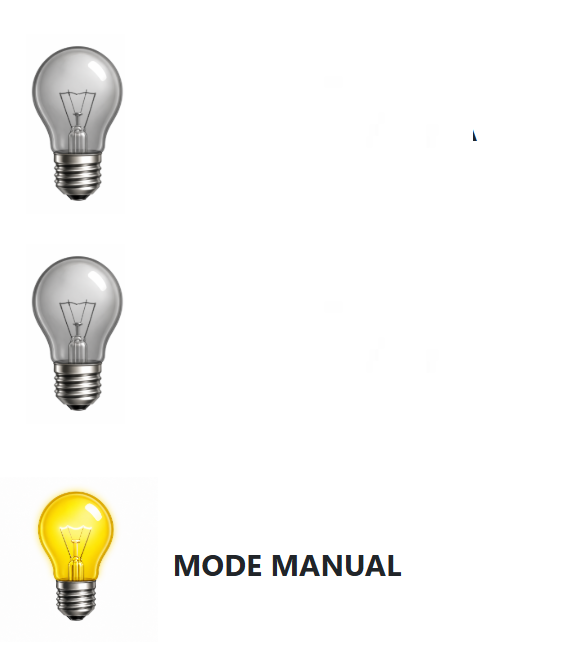
\includegraphics[width=\linewidth]{images/light_manu.png}
    \caption*{Mode manual}
\end{minipage}
\begin{minipage}{0.32\textwidth}
    \centering
    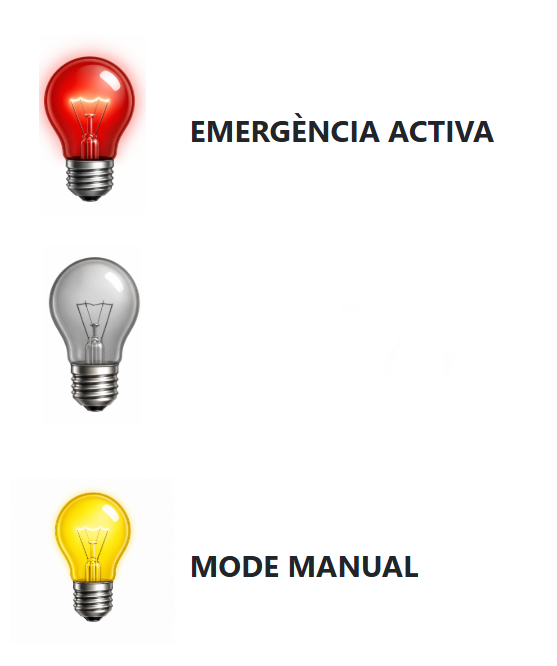
\includegraphics[width=\linewidth]{images/light_emerg.png}
    \caption*{Mode emergència}
\end{minipage}
\caption{Diferents estats dels indicadors de mode}
\label{fig:indicadors_mode}
\end{figure}

\subsection{Vista general de la pantalla}

\begin{figure}[H]
    \centering
    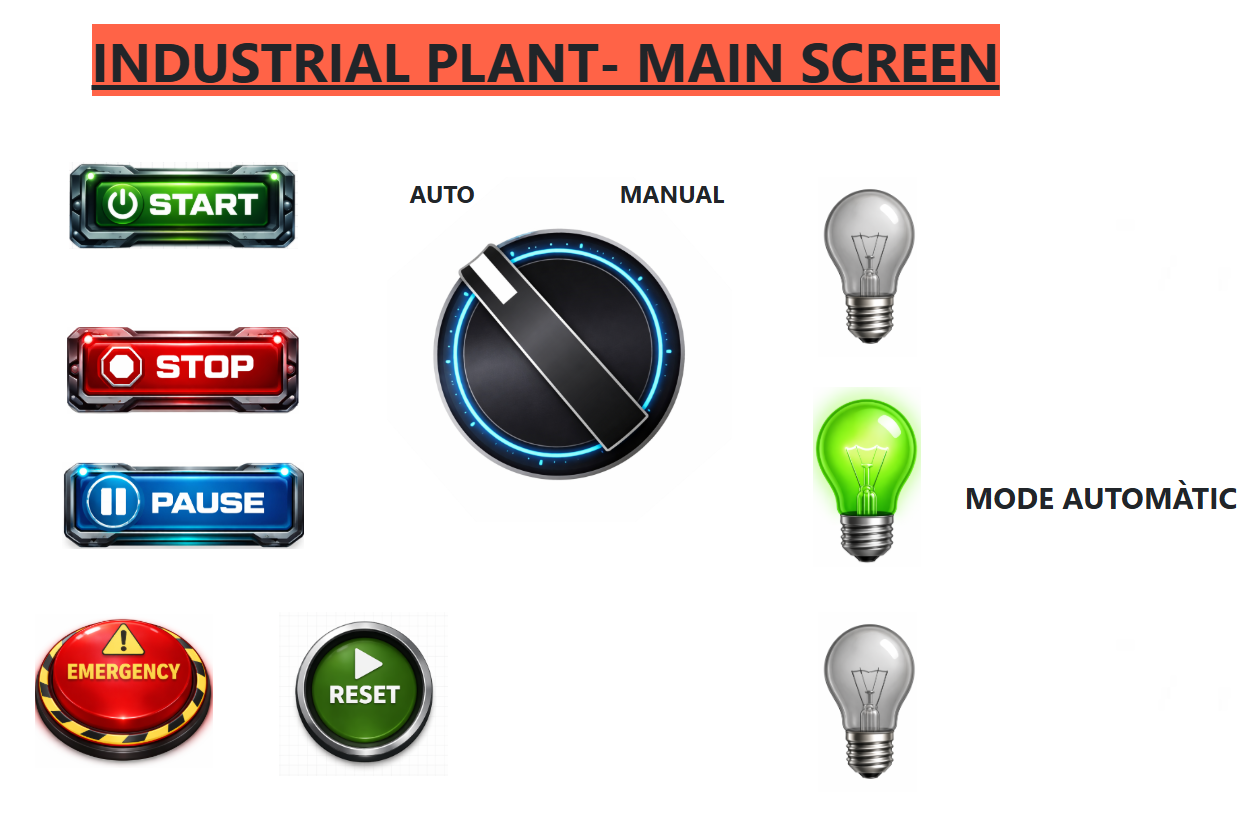
\includegraphics[width=0.9\linewidth]{images/MAIN_SCREEN.png}
    \caption{Pantalla de control del procés}
    \label{fig:main_screen}
\end{figure}

\section{Pantalla de mode manual}

La tercera pantalla està destinada al control manual dels actuadors del sistema (Figura \ref{fig:manual_screen}). També s'ha implementat mitjançant \textit{Mimic Diagram}, degut a la necessitat d'enviar comandes directes. A diferència de les altres pantalles, aquesta no utilitza canals d'entrada, ja que el seu objectiu és únicament enviar comandes al sistema.

\subsection{Control d'actuadors}

Els elements disponibles són:

\begin{itemize}
    \item Cintes transportadores: botons de start/stop que permeten activar o aturar el moviment de la cinta. Quan es prem un botó, s'envia un valor binari (0 o 1) al canal corresponent, que Unity interpreta per iniciar o detenir el desplaçament de les peces.

    \item Rodets de plataformes: tres botons associats a cada sistema de rodets:
    \begin{itemize}
        \item Endavant (valor positiu, habitualment 1)
        \item Enrere (valor negatiu, habitualment -1)
        \item Aturat (valor 0)
    \end{itemize}
    \item Transelevadors: el seu control es basa en l'enviament de \textbf{posicions discretes} en lloc de moviments continus.
    
    Cada transelevador disposa de dos graus de llibertat:
    
    \begin{itemize}
        \item \textbf{Moviment horitzontal:} cada botó envia un valor enter que representa la posició objectiu al llarg dels carrils (per exemple, entre 0 i 3 segons el nombre de posicions disponibles).
        \item \textbf{Moviment vertical:} de manera anàloga, s'envien valors discrets que indiquen el nivell d'alçada desitjat.
    \end{itemize}

Aquests valors són interpretats a Unity com a consignes de posició, encarregant-se el sistema de moure el transelevador fins a la ubicació indicada.

\end{itemize}


\subsection{Vista general de la pantalla}

\begin{figure}[H]
    \centering
    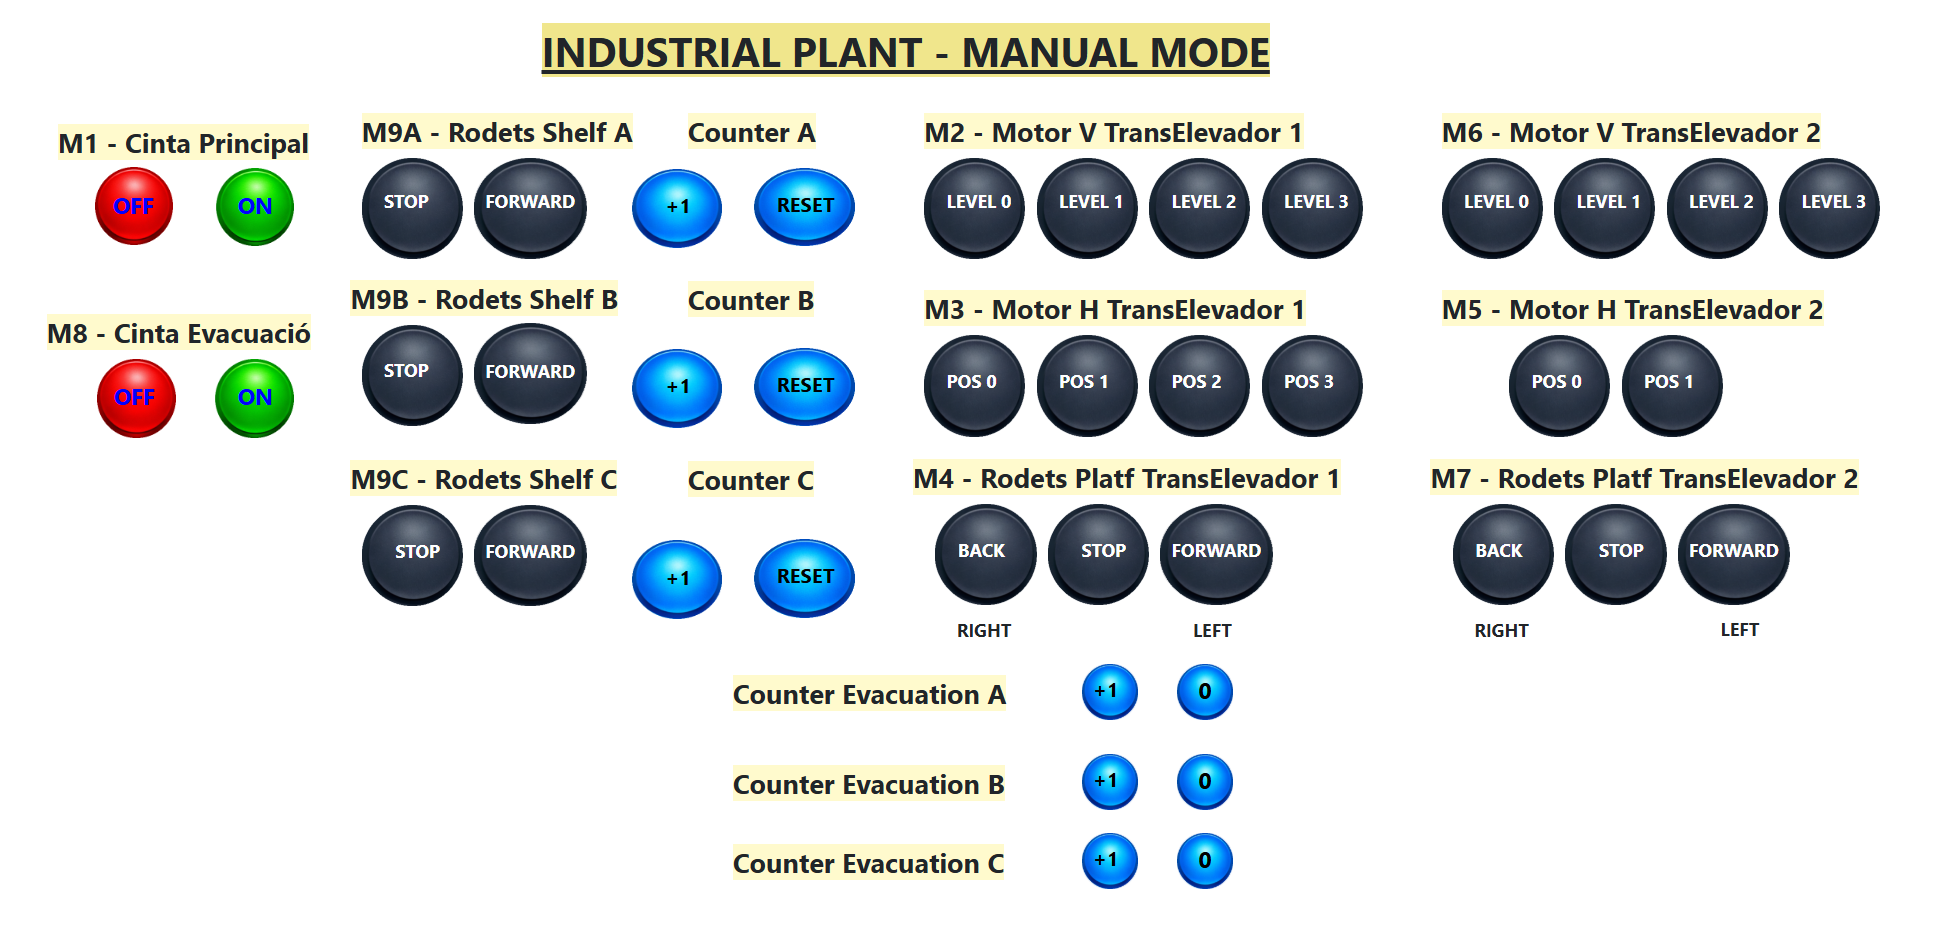
\includegraphics[width=0.9\linewidth]{images/manual_screen.png}
    \caption{Pantalla de control manual}
    \label{fig:manual_screen}
\end{figure}


\section{Pantalla de gràfics i taula general}

Amb l'objectiu de millorar la visualització i anàlisi de les dades del sistema, s'han incorporat dues noves pantalles: una taula general i una pantalla de gràfics.

\subsection{Taula general de dades}

La taula general s'ha implementat mitjançant una vista de tipus \texttt{.tbl}, que permet visualitzar tots els canals configurats dins del sistema.

Aquesta vista presenta les següents característiques:
\begin{itemize}
    \item Visualització en temps real dels canals d'entrada (\textit{input channels})
    \item Possibilitat d'enviar comandes als canals de sortida (\textit{output channels})
    \item Accés directe a les dades històriques
\end{itemize}

Aquesta taula constitueix una eina útil tant per a la supervisió com per al test del sistema.

\subsection{Visualització de gràfics amb Chart Pro}

Per a la representació gràfica de dades, s'ha utilitzat el plugin \textbf{Chart Pro} \cite{rapidscada_chart_pro}, que amplia les funcionalitats del sistema base (Figura \ref{fig:tabla_grafico}).

Les millores principals que aporta són:
\begin{itemize}
    \item Visualització de múltiples canals en un mateix gràfic
    \item Comparació simultània de variables
    \item Exportació de gràfics i dades en formats com PDF o PNG
\end{itemize}

A diferència del sistema base, que només permet visualitzar un canal per gràfic, aquest plugin facilita una anàlisi més completa del comportament del sistema.


\begin{figure}[H]
\centering
\begin{minipage}{0.48\textwidth}
    \centering
    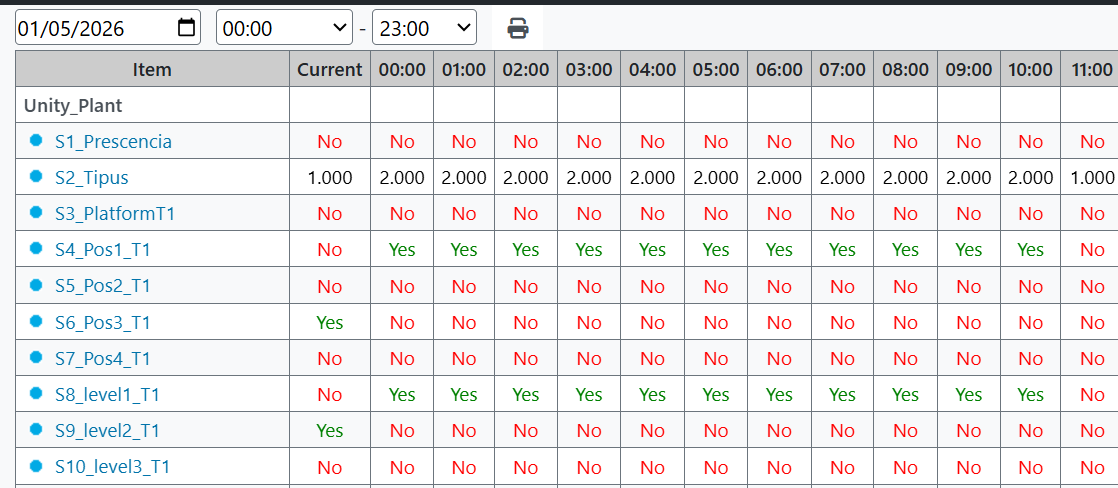
\includegraphics[width=\linewidth]{images/tabla_general.png}
    \caption*{Vista parcial de la taula de dades}
\end{minipage}
\hfill
\begin{minipage}{0.48\textwidth}
    \centering
    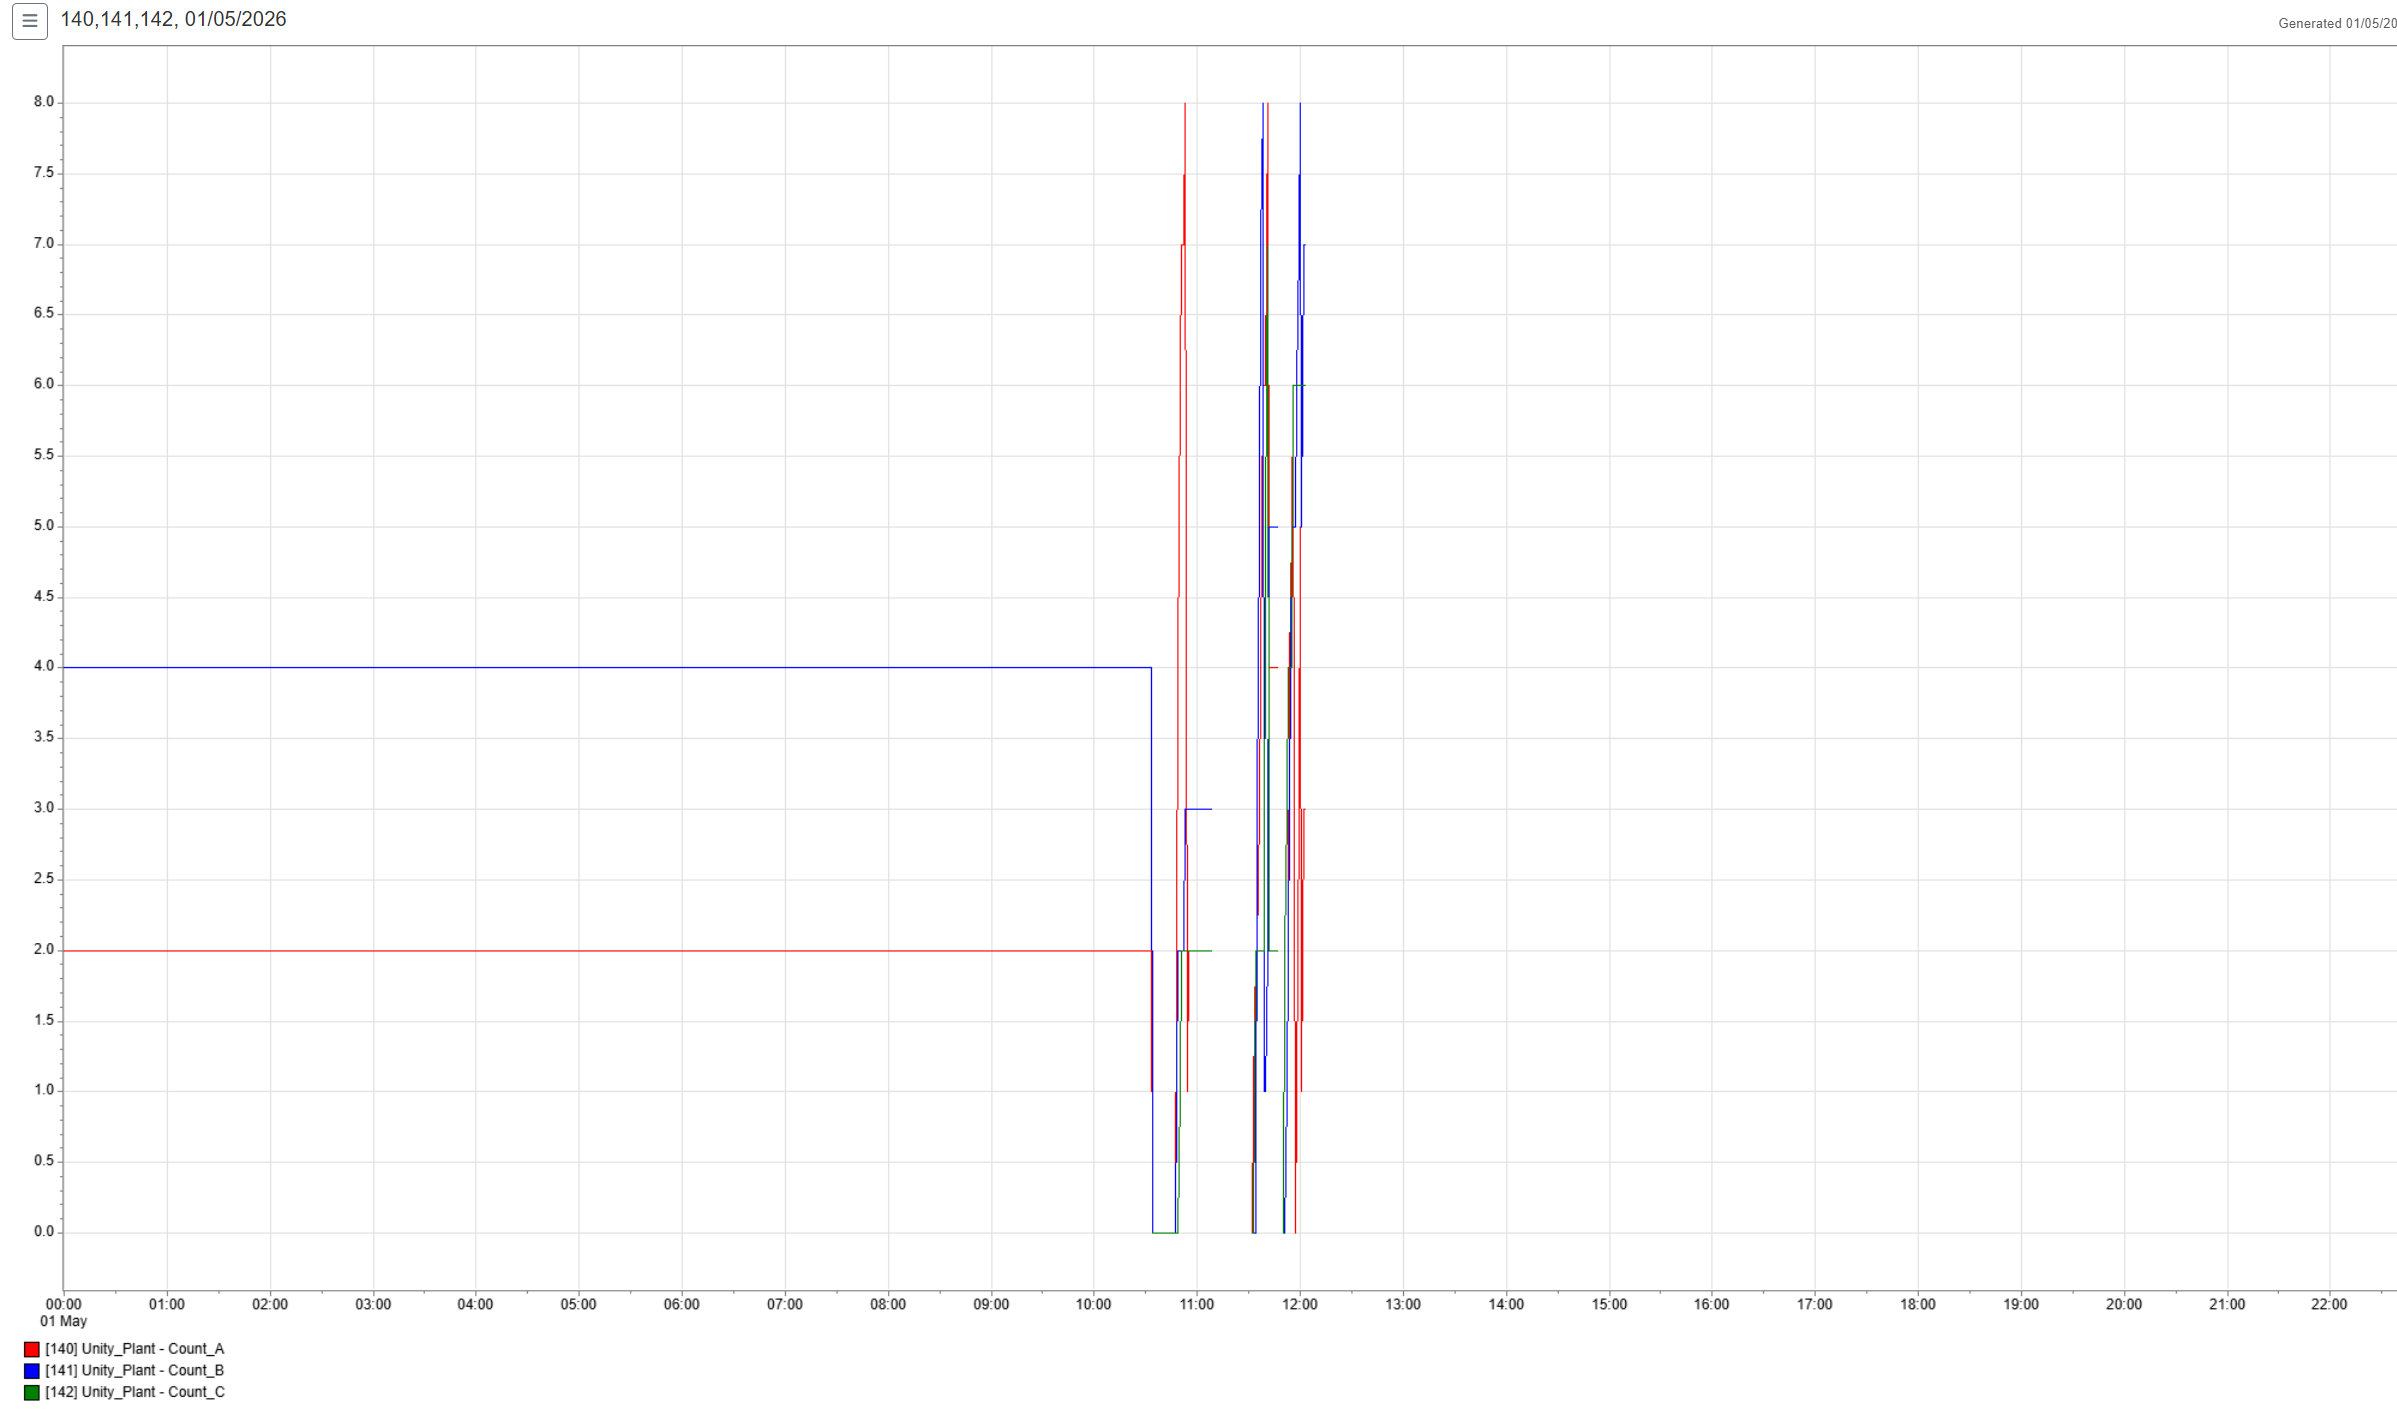
\includegraphics[width=\linewidth]{images/grafico_tabla.png}
    \caption*{Gràfic generat a partir de  les variables dels comptadors d'evacuació}
\end{minipage}
\caption{Relació entre la visualització tabular i la representació gràfica de dades}
\label{fig:tabla_grafico}
\end{figure}


La vista en format taula permet accedir directament als valors de les variables, mentre que la selecció d'un canal concret facilita la generació de gràfics per a l'anàlisi de la seva evolució temporal.

\subsection{Integració de gràfics en esquemes}

Addicionalment, s'ha creat una pantalla de tipus \texttt{.sch} utilitzant el plugin \textit{Extra Scheme Editor}, que permet integrar gràfics directament dins dels esquemes visuals.

En aquest cas, s'ha implementat un gràfic (Figura \ref{fig:grafico_esquema}) que mostra les variables de comptador d'evacuació (EvacA, EvacB i EvacC), amb l'objectiu de comparar el rendiment del sistema.

Cal destacar que els gràfics integrats en fitxers \texttt{.sch} presenten certes limitacions en comparació amb els gràfics generats des de les vistes de tipus \texttt{.tbl} els quals, en seleccionar una variable, ofereixen funcionalitats més avançades, com:
\begin{itemize}
    \item Selecció d'intervals de temps
    \item Visualització detallada de l'evolució de la variable
    \item Major capacitat d'anàlisi de dades
\end{itemize}

Per tant, els gràfics en esquemes són útils per a una visualització integrada i immediata, mentre que les vistes \texttt{.tbl} resulten més adequades per a l'anàlisi detallada del sistema.

Cal destacar també que la correcta configuració de Chart Pro és necessària per visualitzar múltiples canals. En cas contrari, només es mostrarà un únic canal. A més, aquest plugin requereix una llicència (trial o permanent). De la mateixa manera passa amb el \textit{ExtraSchemeEditor}, que és necessari per veure el gràfic en aquesta mateixa pantalla, sinó l'única manera de visualitzar els gràfics és a través de la taula.


\begin{figure}[H]
    \centering
    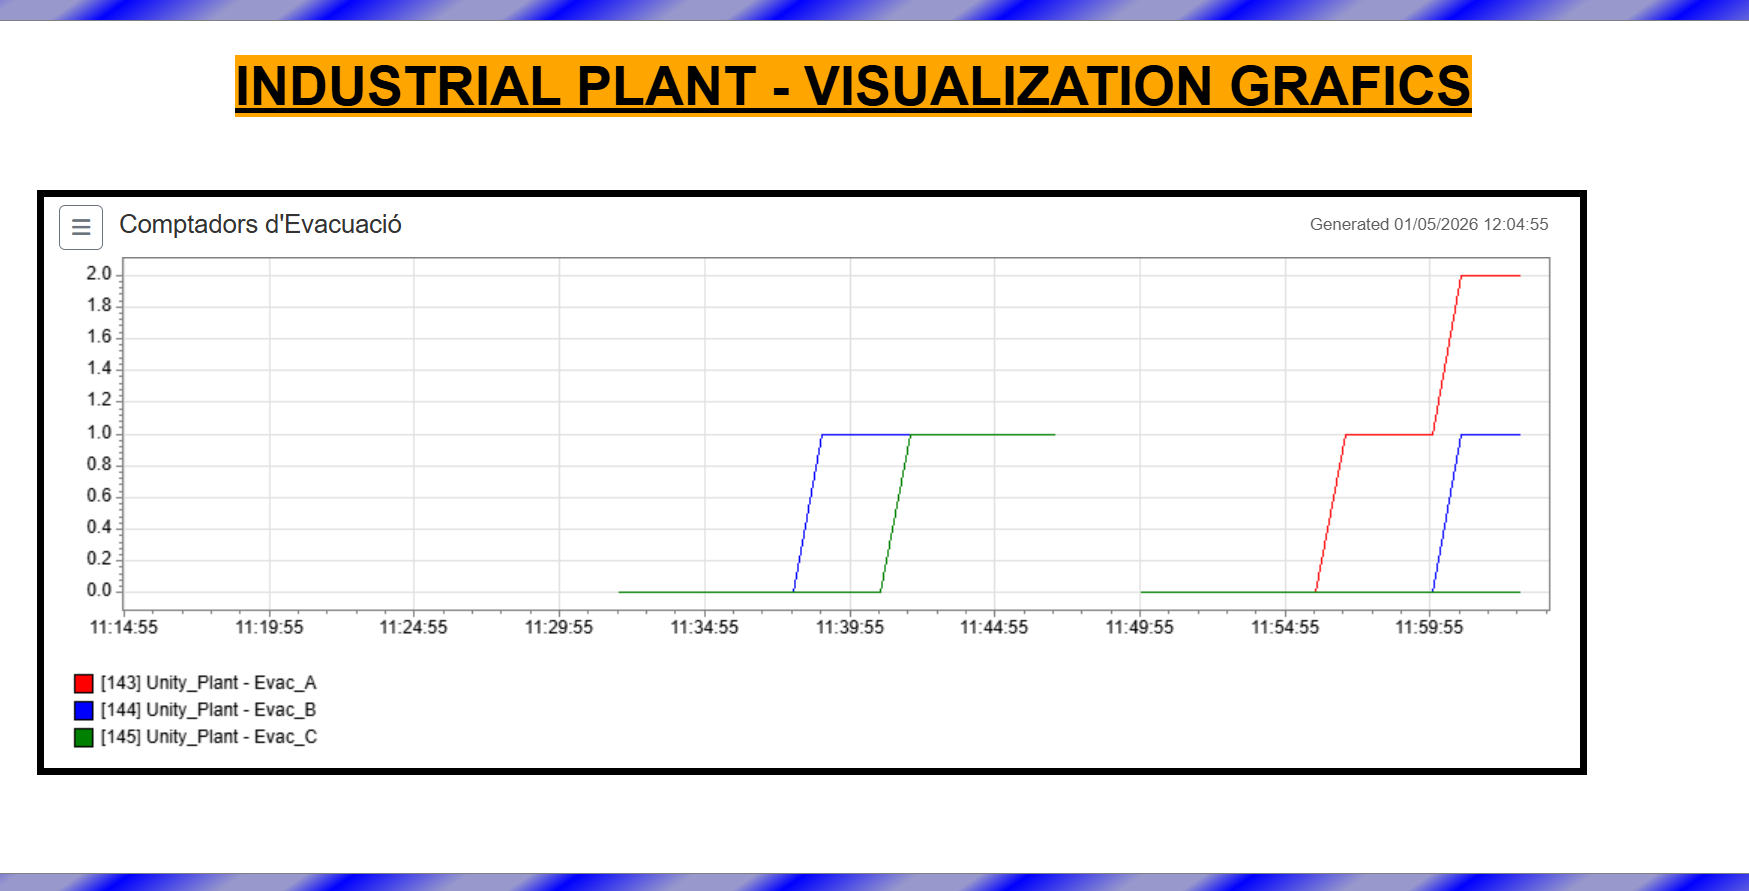
\includegraphics[width=0.8\linewidth]{images/grafico_esquema.png}
    \caption{Gràfic integrat dins d'un esquema utilitzant Extra Scheme Editor}
    \label{fig:grafico_esquema}
\end{figure}

\section{Configuració d'usuaris i control d'accés}

Per tal de gestionar correctament l'accés a les diferents funcionalitats del sistema, s'ha implementat un sistema de control basat en rols i permisos (Figura \ref{fig:objects_scada}).

\subsection{Definició de rols}

S'han creat tres rols principals \cite{rapidscada_user_management}:  
\begin{itemize}
    \item \textbf{Supervisor}: accés complet al sistema
    \item \textbf{Operator}: accés parcial amb capacitat de control limitada
    \item \textbf{User}: accés únicament de visualització
\end{itemize}

\begin{figure}[H]
    \centering
    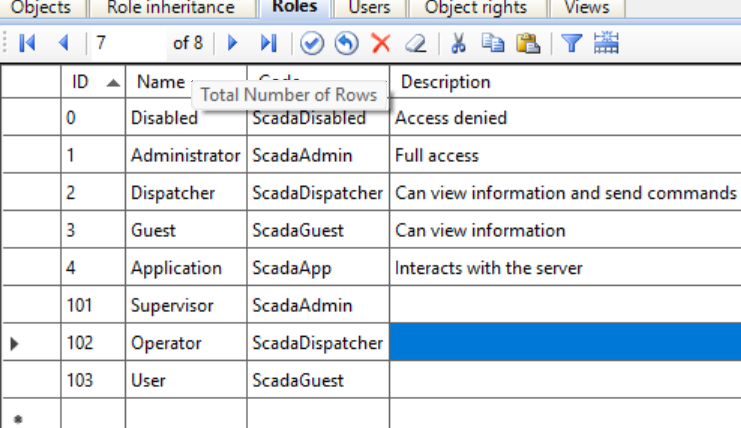
\includegraphics[width=0.5\linewidth]{images/rols_scada.png}
    \caption{Rols en RapidScada}
    \label{fig:rols_scada}
\end{figure}

\subsection{Organització de les pantalles}

Les pantalles del sistema s'han organitzat en diferents categories amb l'objectiu de facilitar la gestió dels permisos d'accés mitjançant els \textit{Object rights} de Rapid SCADA (Figura \ref{fig:objects_scada}):

\begin{itemize}
    \item \textbf{Mode}: inclou les vistes generals del sistema (Vista\_Planta.tbl i MainScreen.mim)
    \item \textbf{Manual}: pantalla de control manual dels actuadors (ModeManual.mim)
    \item \textbf{Gràfics}: visualització de dades històriques (Grafics.sch)
    \item \textbf{Visualització}: pantalla de visualització de sensors, motors i comptadors (Visualization.sch)
\end{itemize}


Aquests grups permeten assignar permisos de forma estructurada mitjançant la configuració de \textit{Object rights}.

\begin{figure}[H]
\centering
\begin{minipage}{0.5\textwidth}
    \centering
    \includegraphics[width=\linewidth]{images/objects_scada.png}
    \caption*{Creació objectes}
\end{minipage}
\hfill
\begin{minipage}{0.7\textwidth}
    \centering
    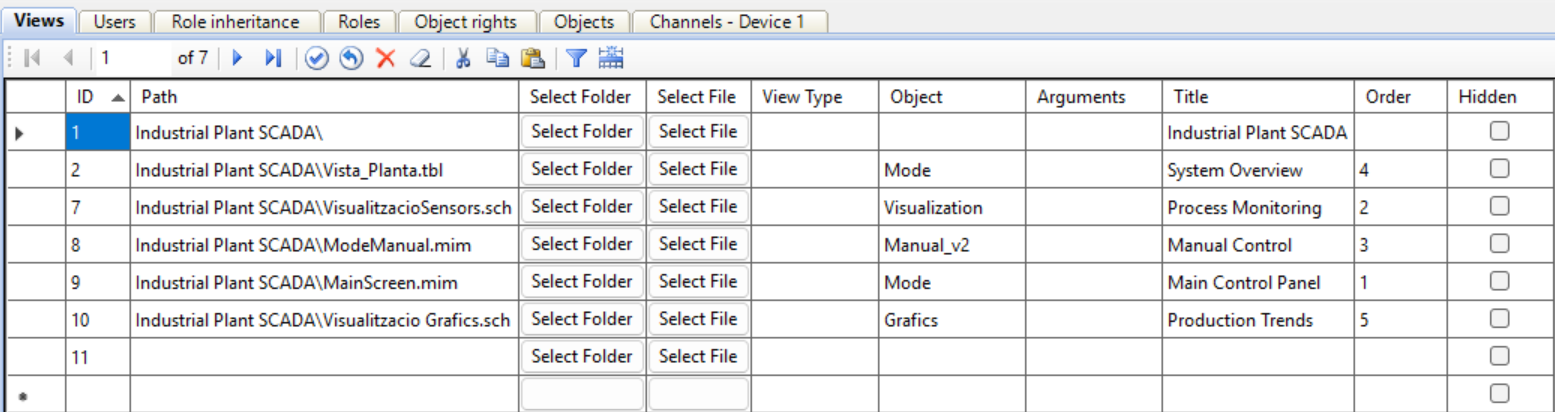
\includegraphics[width=\linewidth]{images/views_scada.png}
    \caption*{Assignació objectes}
\end{minipage}
\caption{Taules referents a objectes en RapidScada}
\label{fig:objects_scada}
\end{figure}
\subsection{Assignació de permisos}

Els permisos s'han distribuït de la següent manera (Figura \ref{fig:objectsrights_scada}):
\begin{itemize}
    \item \textbf{Supervisor}: accés complet a totes les pantalles i funcionalitats, amb permisos de \textit{View} i \textit{Control} en tots els casos.

    \item \textbf{Operator}: accés a la majoria de pantalles amb permisos de visualització en tots els modes, però amb capacitat de control restringida únicament a la pantalla de mode manual.

    \item \textbf{User}: accés limitat exclusivament a la visualització de dades, sense capacitat d'interacció amb el sistema.
\end{itemize}
\begin{figure}[H]
    \centering
    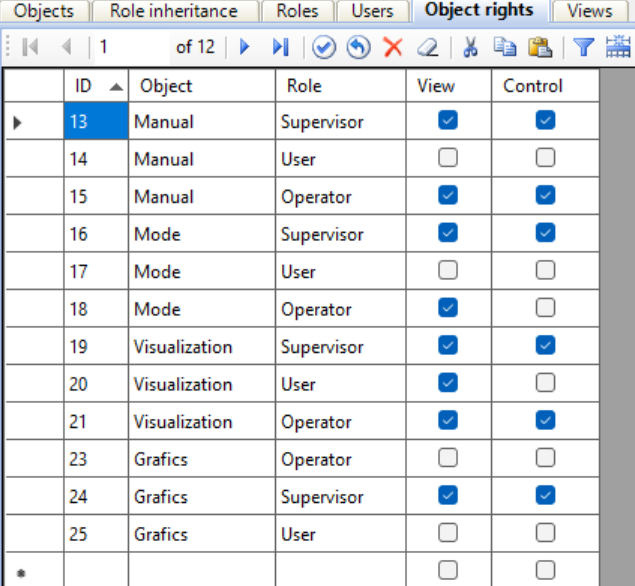
\includegraphics[width=0.32\linewidth]{images/objectsrights_scada.png}
    \caption{Assignació objectes a rols en RapidScada}
    \label{fig:objectsrights_scada}
\end{figure}

\subsection{Creació d'usuaris}

S'han creat diferents usuaris associats als rols definits, cadascun amb les seves credencials d'accés. Per tal de simplificar la gestió, els noms dels usuaris coincideixen amb els rols corresponents.

La configuració de les credencials es realitza des de l'eina d'administració de Rapid SCADA, on es poden definir les contrasenyes i assignar els rols de manera individual.

Cal destacar que Rapid SCADA inclou usuaris i rols predefinits (com l'usuari \textit{Admin}), que també poden ser utilitzats dins del sistema. En aquells casos en què no es defineixen explícitament permisos de \textit{View} o \textit{Control}, el comportament per defecte vindrà determinat per la configuració interna del sistema. (CITAR SECCION USUARIOS RAPIDSCADA)

\end{document}